\chapter{Adversarial, Runtime \& Spacetime Charts (Studies 02, 03 \& 06)}
\label{appendix:fairness-scalability-charts}

This appendix collects the evaluation plots for Studies~02, 03, and~06 (Section~\ref{sec:fairness-computational-rigour}). Numeric tables and interpretation remain in the main evaluation chapter; the figures are deferred here to reduce clutter.

\begin{figure}[htbp]
    \centering
    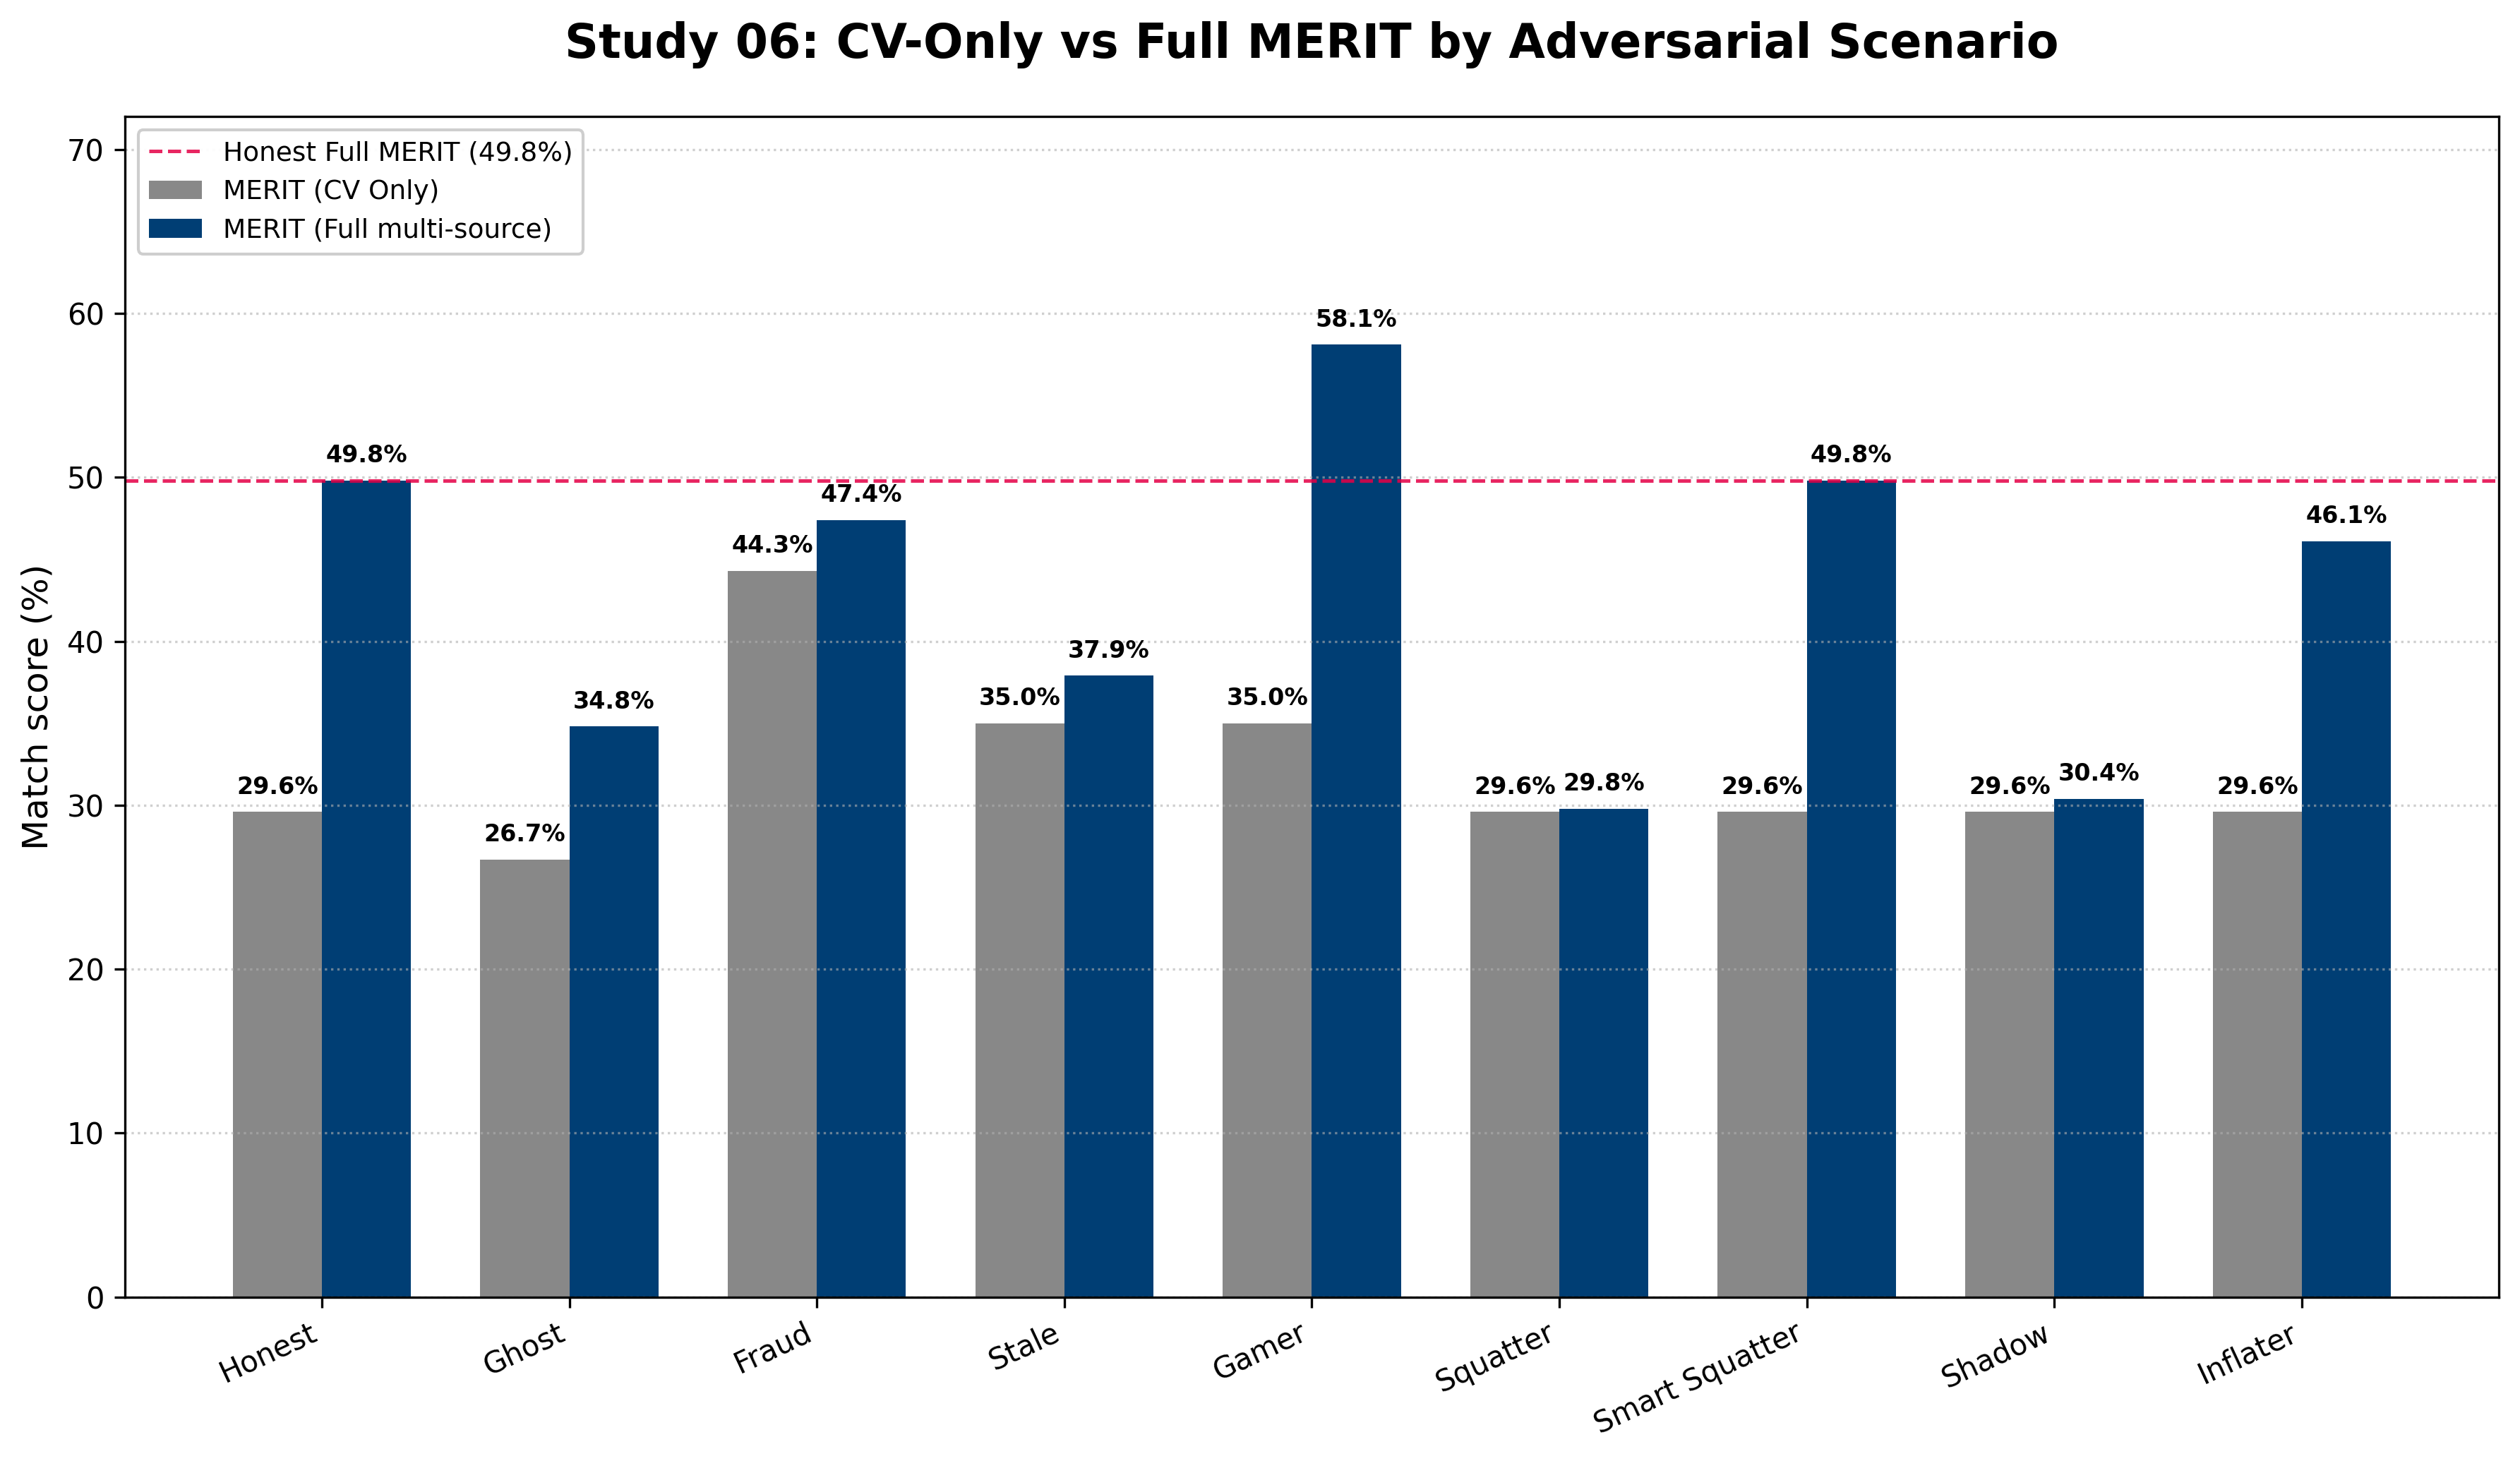
\includegraphics[width=0.95\textwidth]{../evaluation/06-adversarial_test/output/adversarial_cv_vs_full.png}
    \caption{Study~06: CV-only versus Full MERIT match scores for each adversarial scenario. Grey bars use the CV only; navy bars add GitHub and LinkedIn fusion. The dashed line marks the honest Full MERIT baseline (49.8\%).}
    \label{fig:adversarial-cv-vs-full}
\end{figure}

\begin{figure}[htbp]
    \centering
    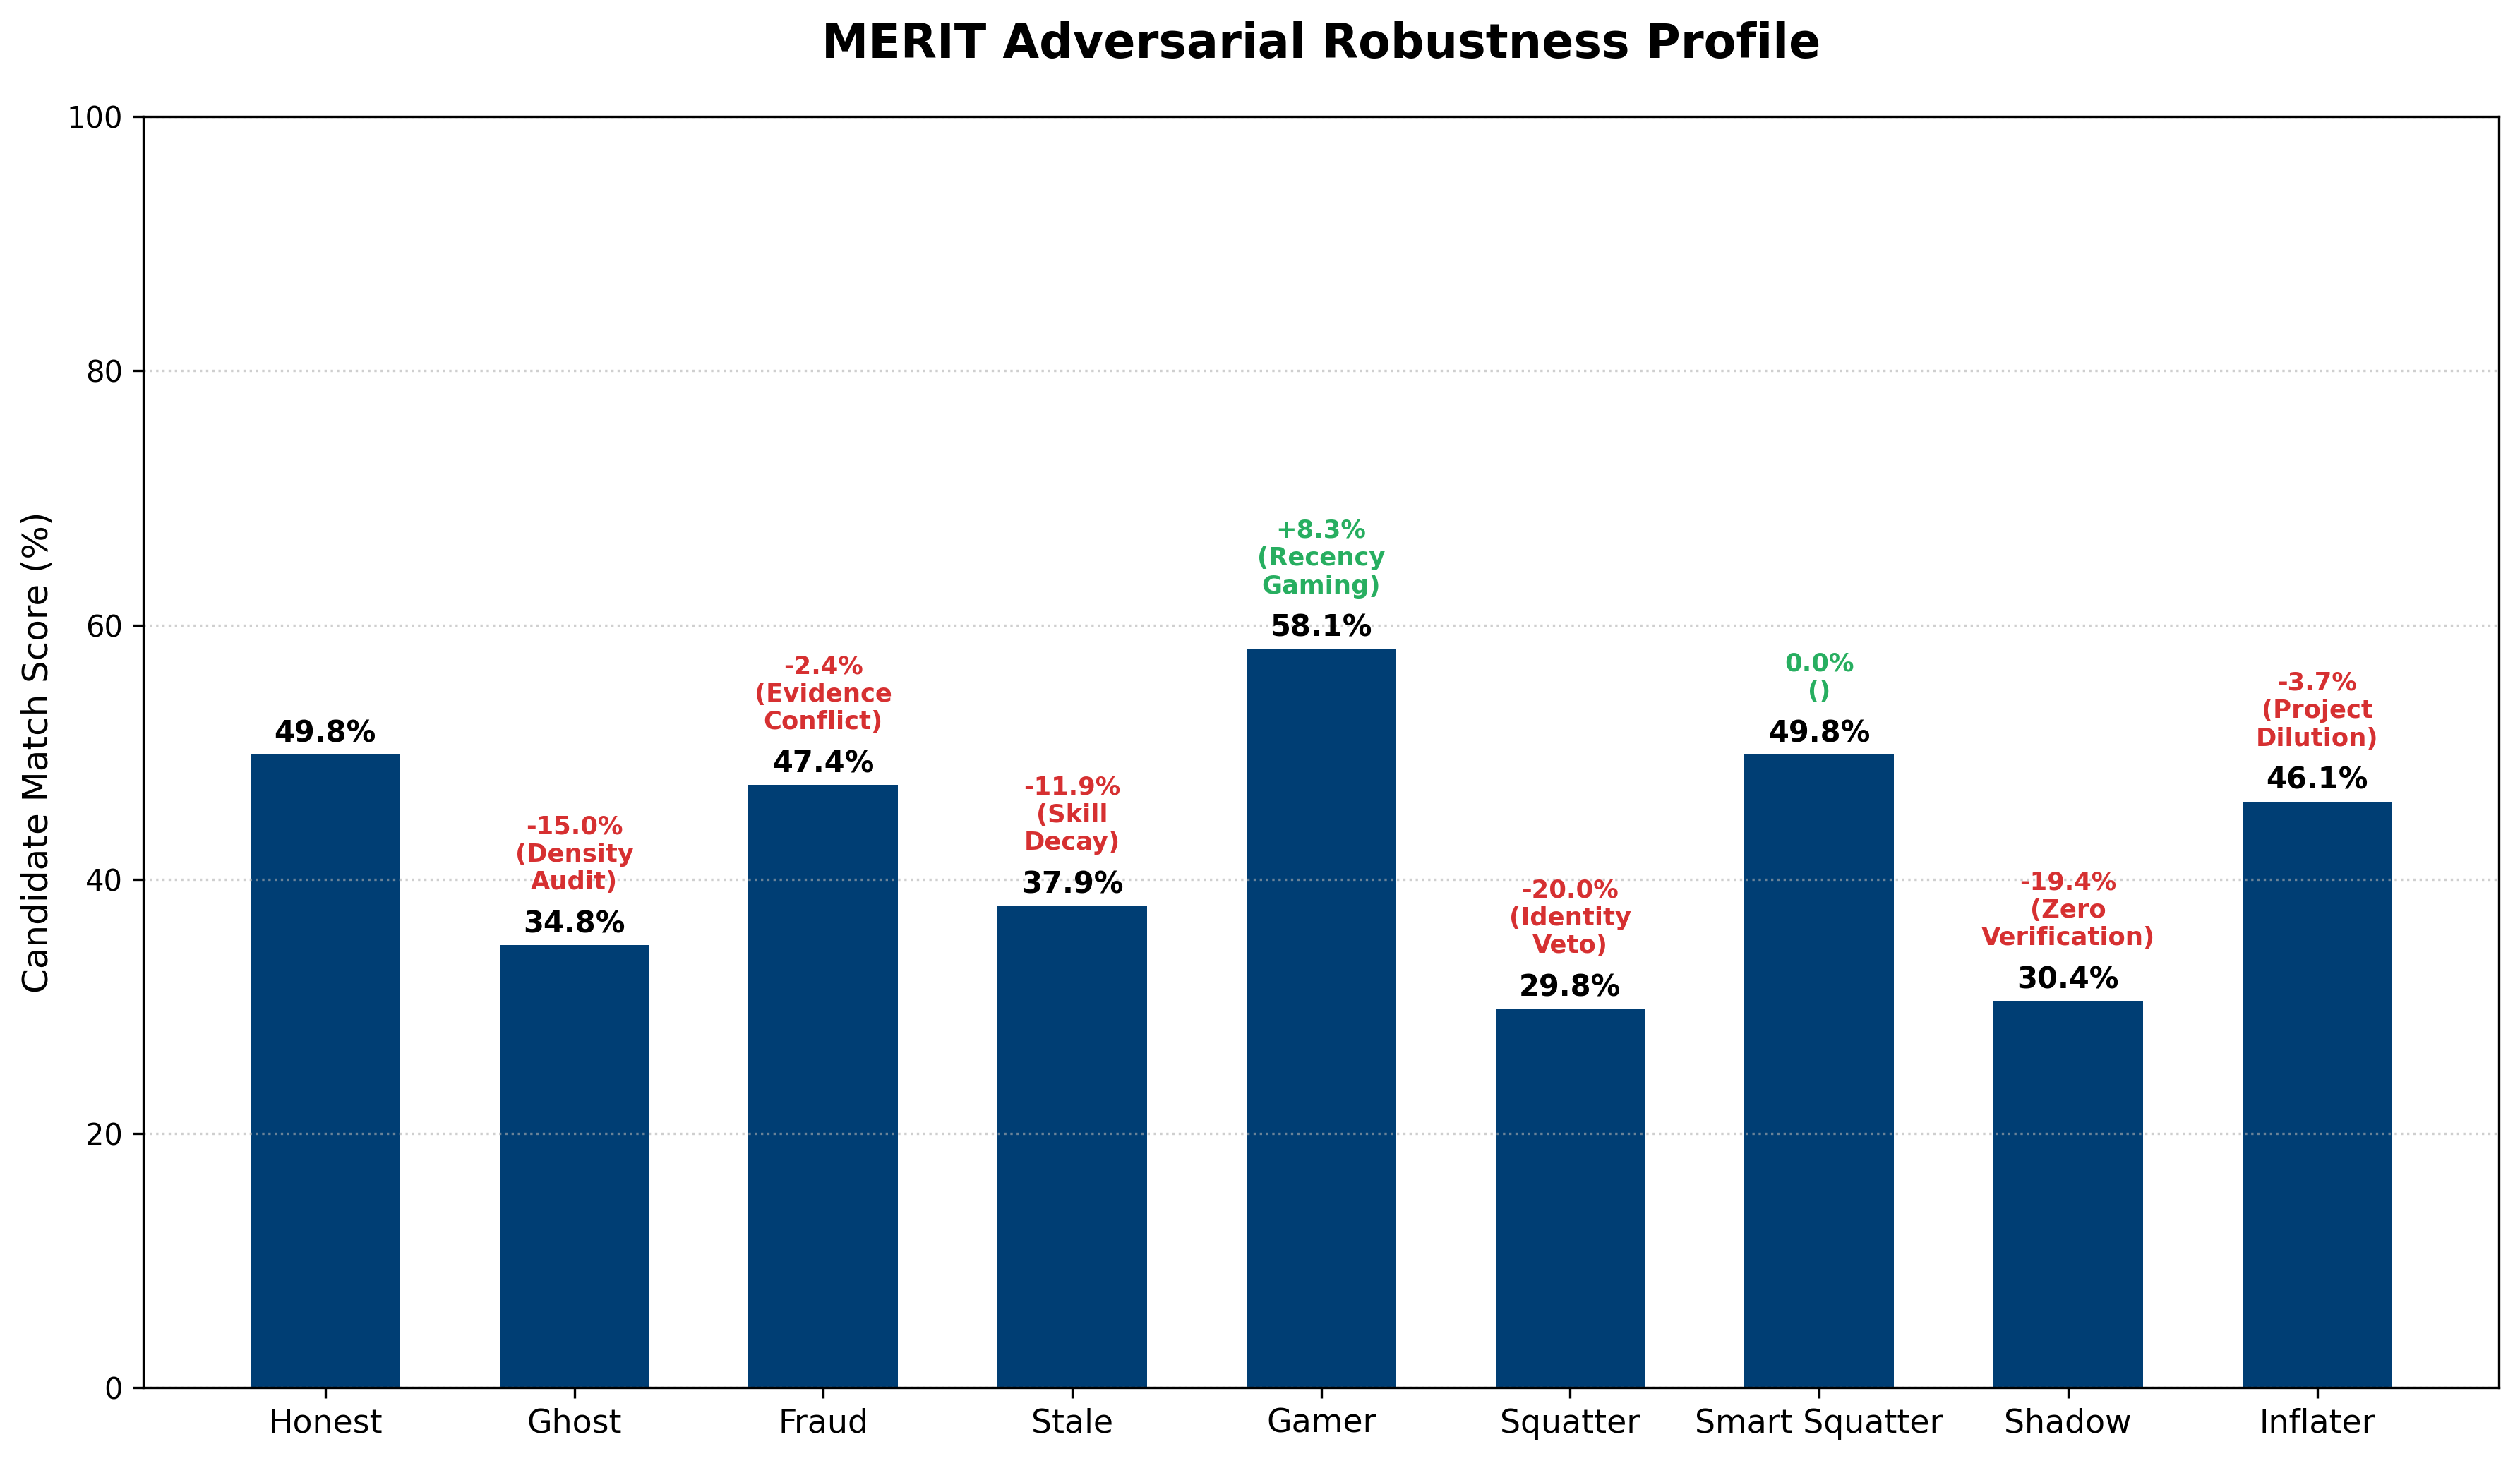
\includegraphics[width=0.95\textwidth]{../evaluation/06-adversarial_test/output/adversarial_robustness.png}
    \caption{MERIT adversarial robustness profile (Study~06). Bars show Full MERIT scores; annotations report $\Delta_{\mathrm{honest\_fusion}}$ (vs.\ honest Full 49.8\%) and the dominant mitigation or failure mechanism (Table~\ref{tab:adversarial-matrix}).}
    \label{fig:adversarial-robustness}
\end{figure}

\begin{figure}[htbp]
    \centering
    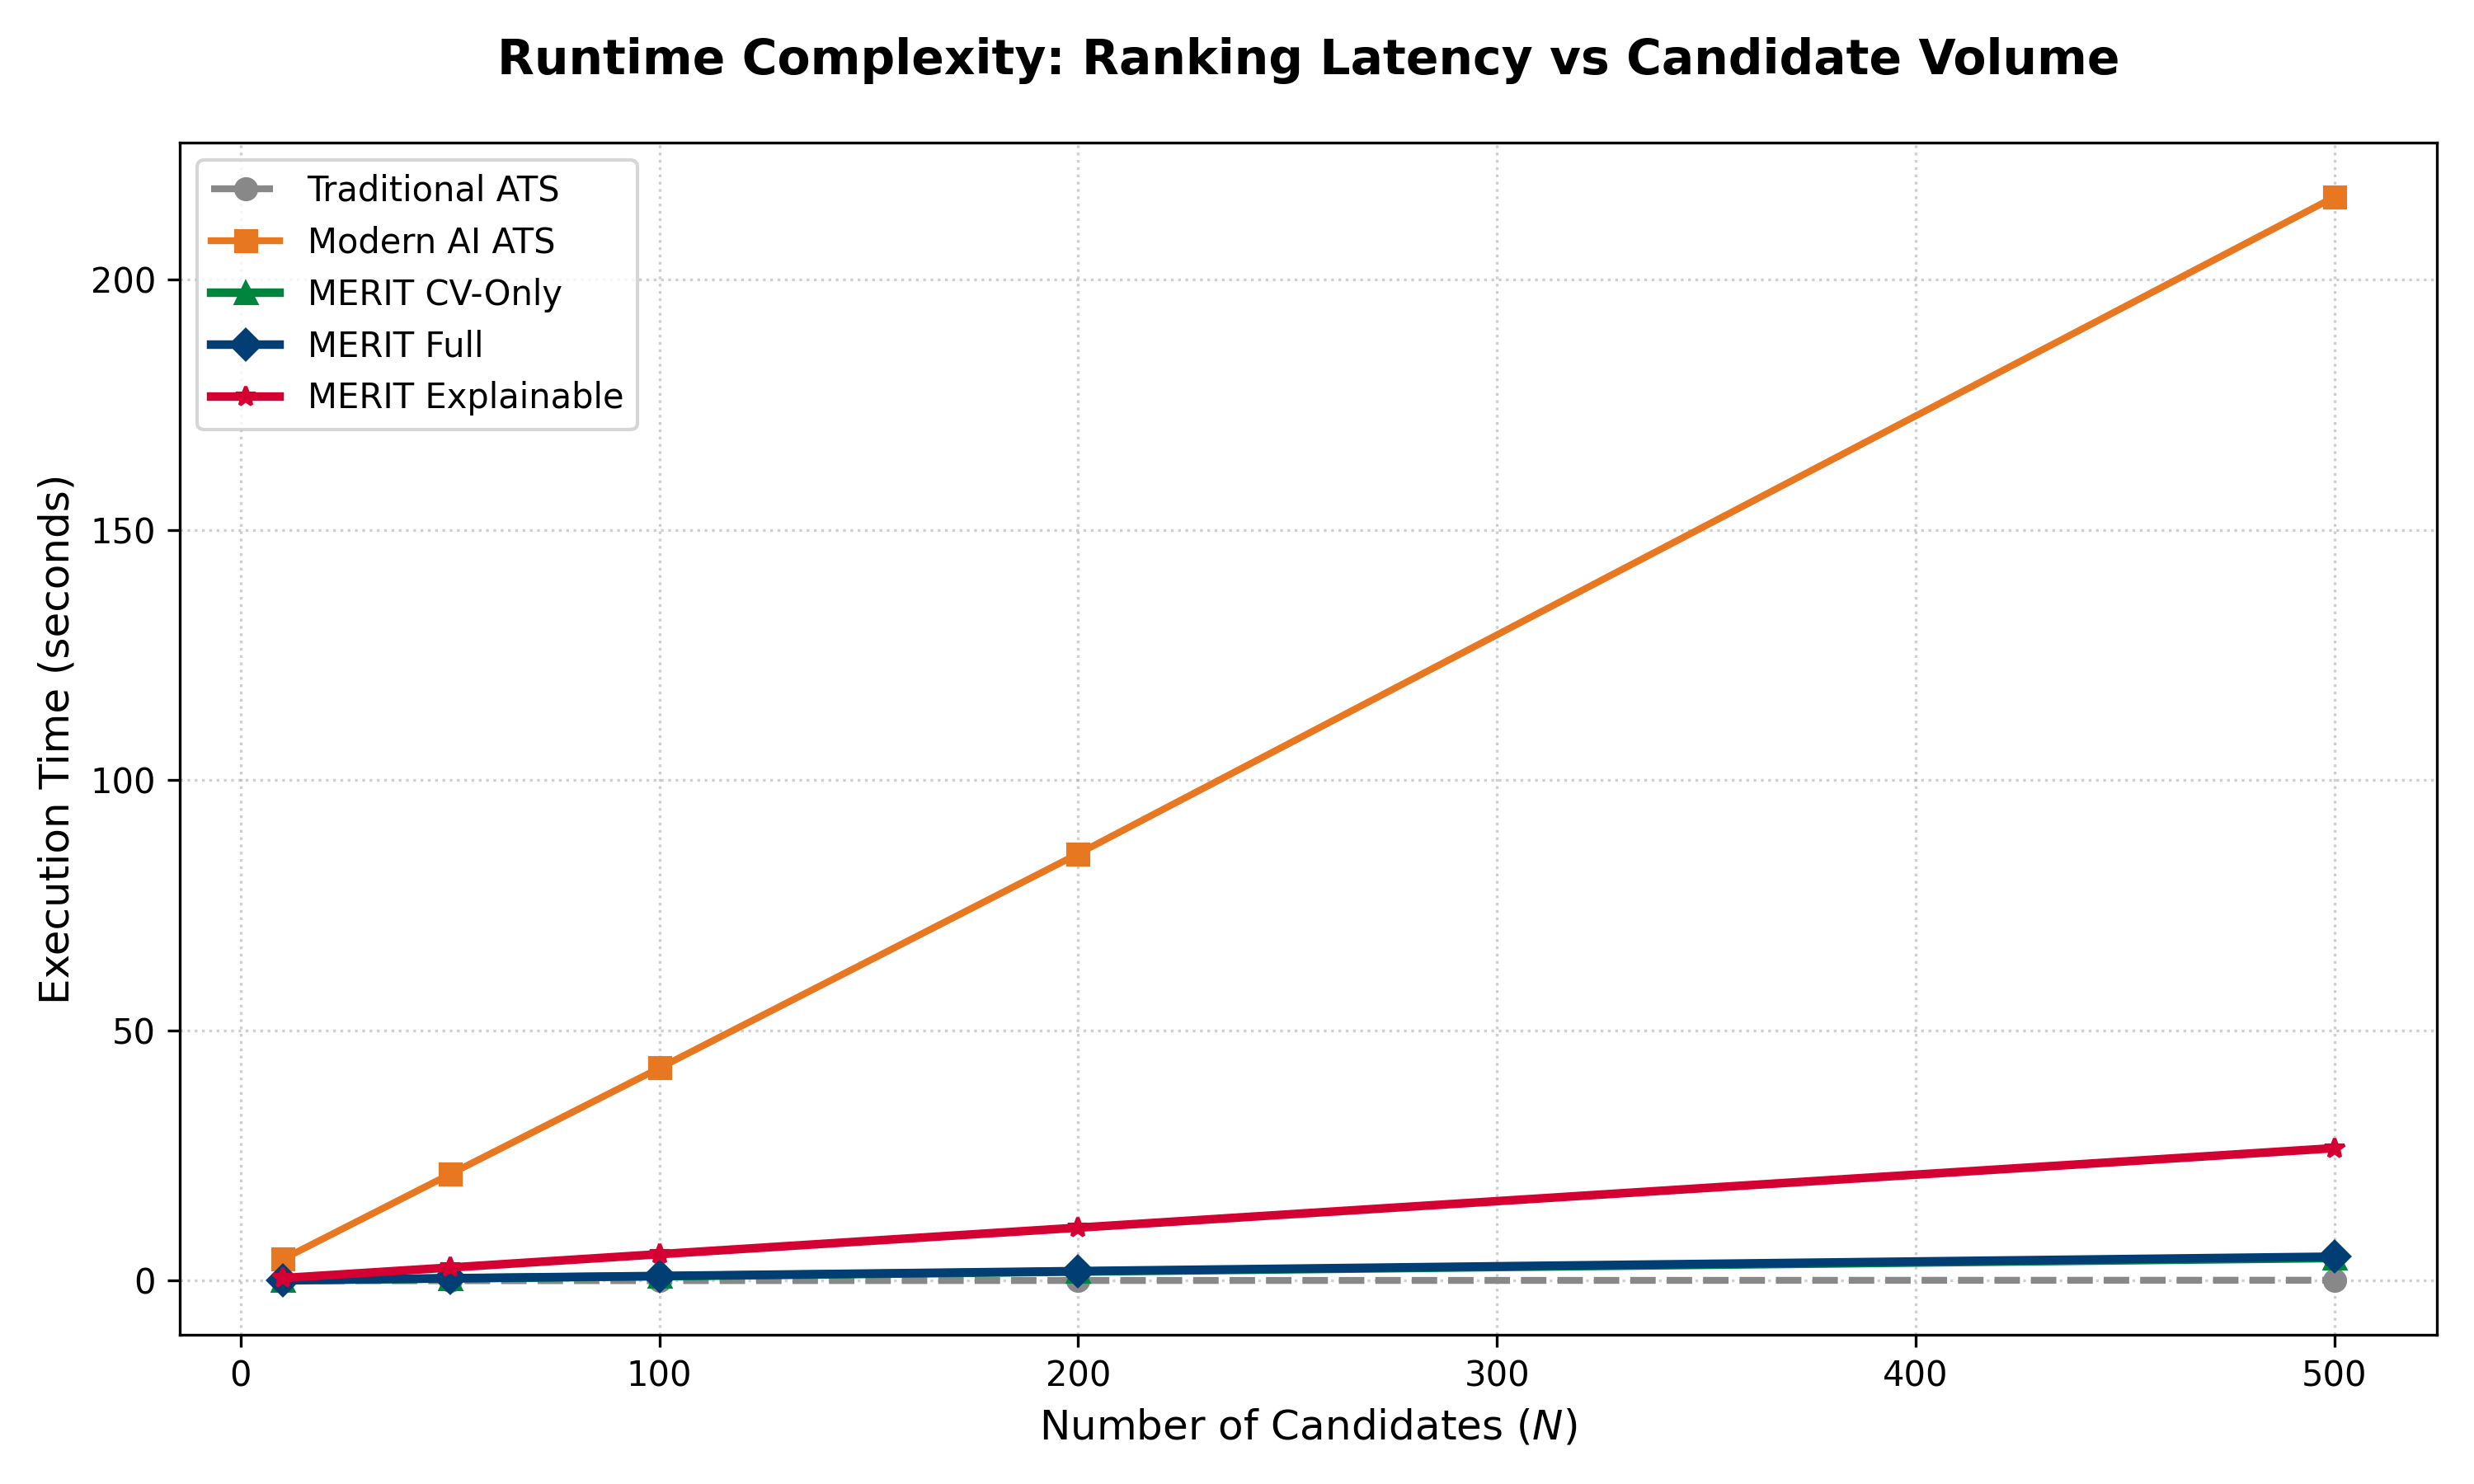
\includegraphics[width=0.92\textwidth]{../evaluation/02-runtime_study/output/runtime_complexity_plot.png}
    \caption{Runtime complexity: batch latency vs.\ candidate volume (Study~02). MERIT Full scales linearly with a low constant factor; Modern AI ATS scales linearly but with SBERT-dominated overhead.}
    \label{fig:runtime-complexity}
\end{figure}

\begin{figure}[htbp]
    \centering
    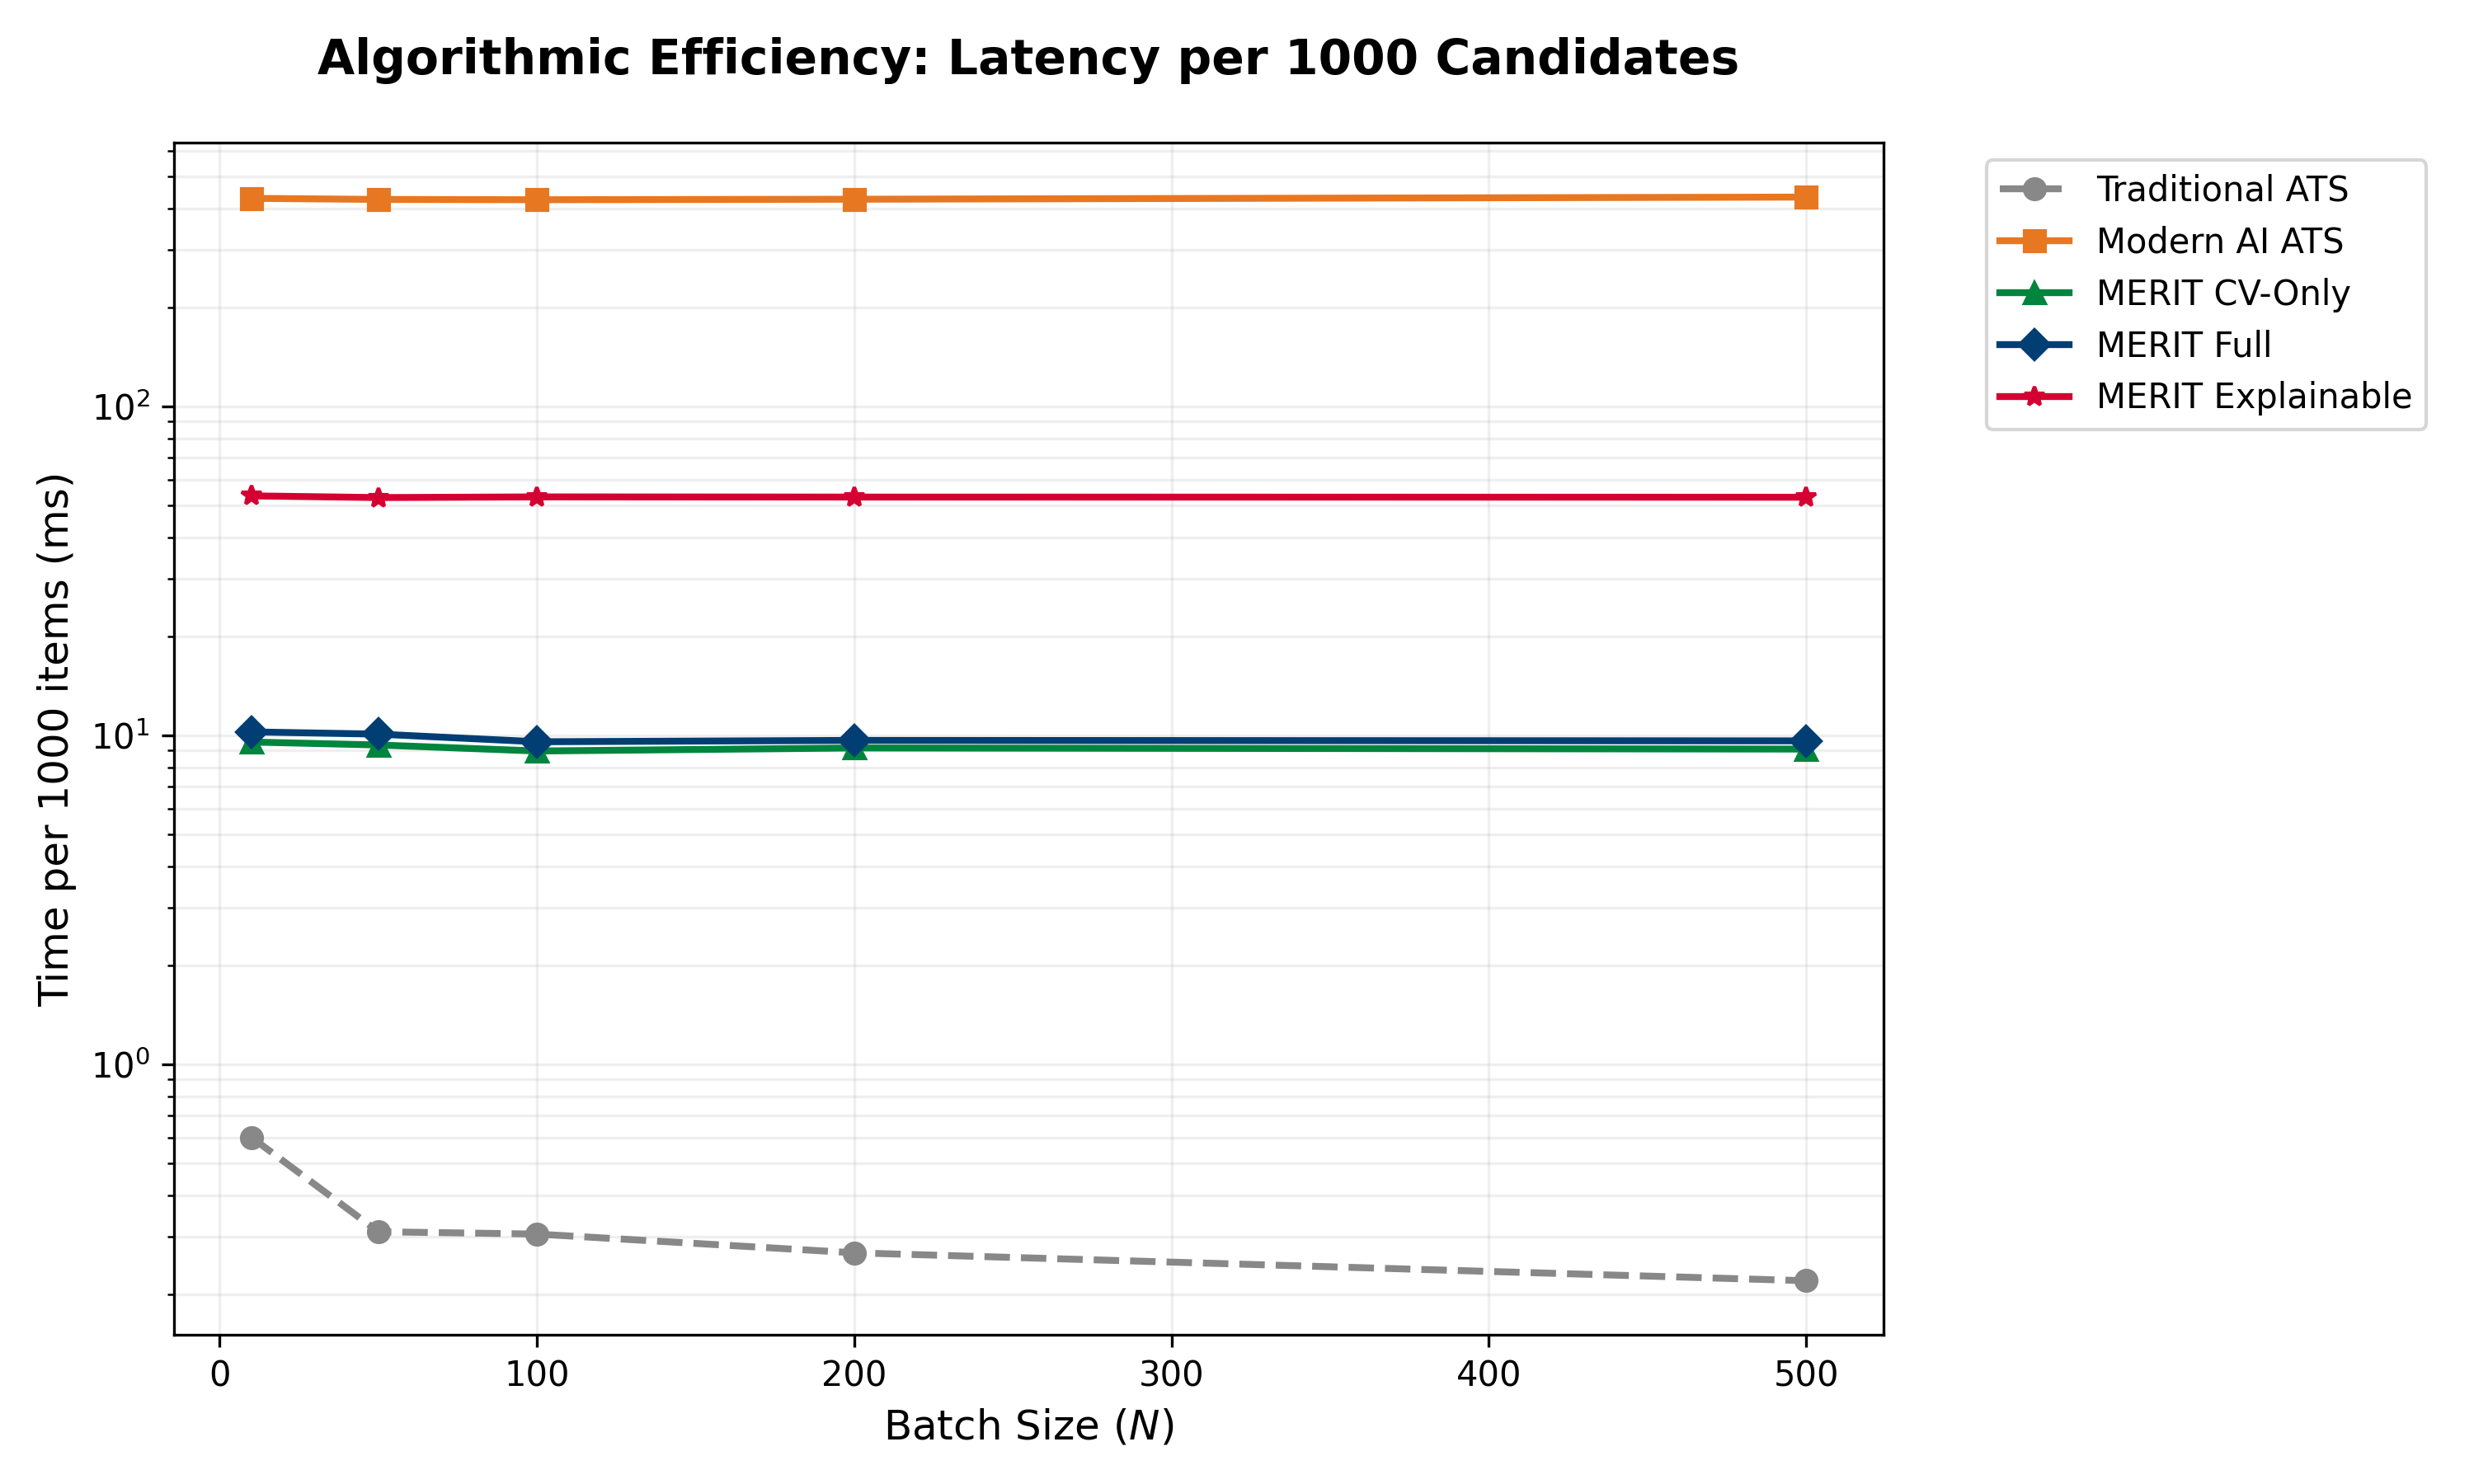
\includegraphics[width=0.92\textwidth]{../evaluation/02-runtime_study/output/runtime_efficiency_log.png}
    \caption{Algorithmic efficiency: normalised latency per 1000 candidates on a log scale (Study~02).}
    \label{fig:runtime-efficiency}
\end{figure}

\begin{figure}[htbp]
    \centering
    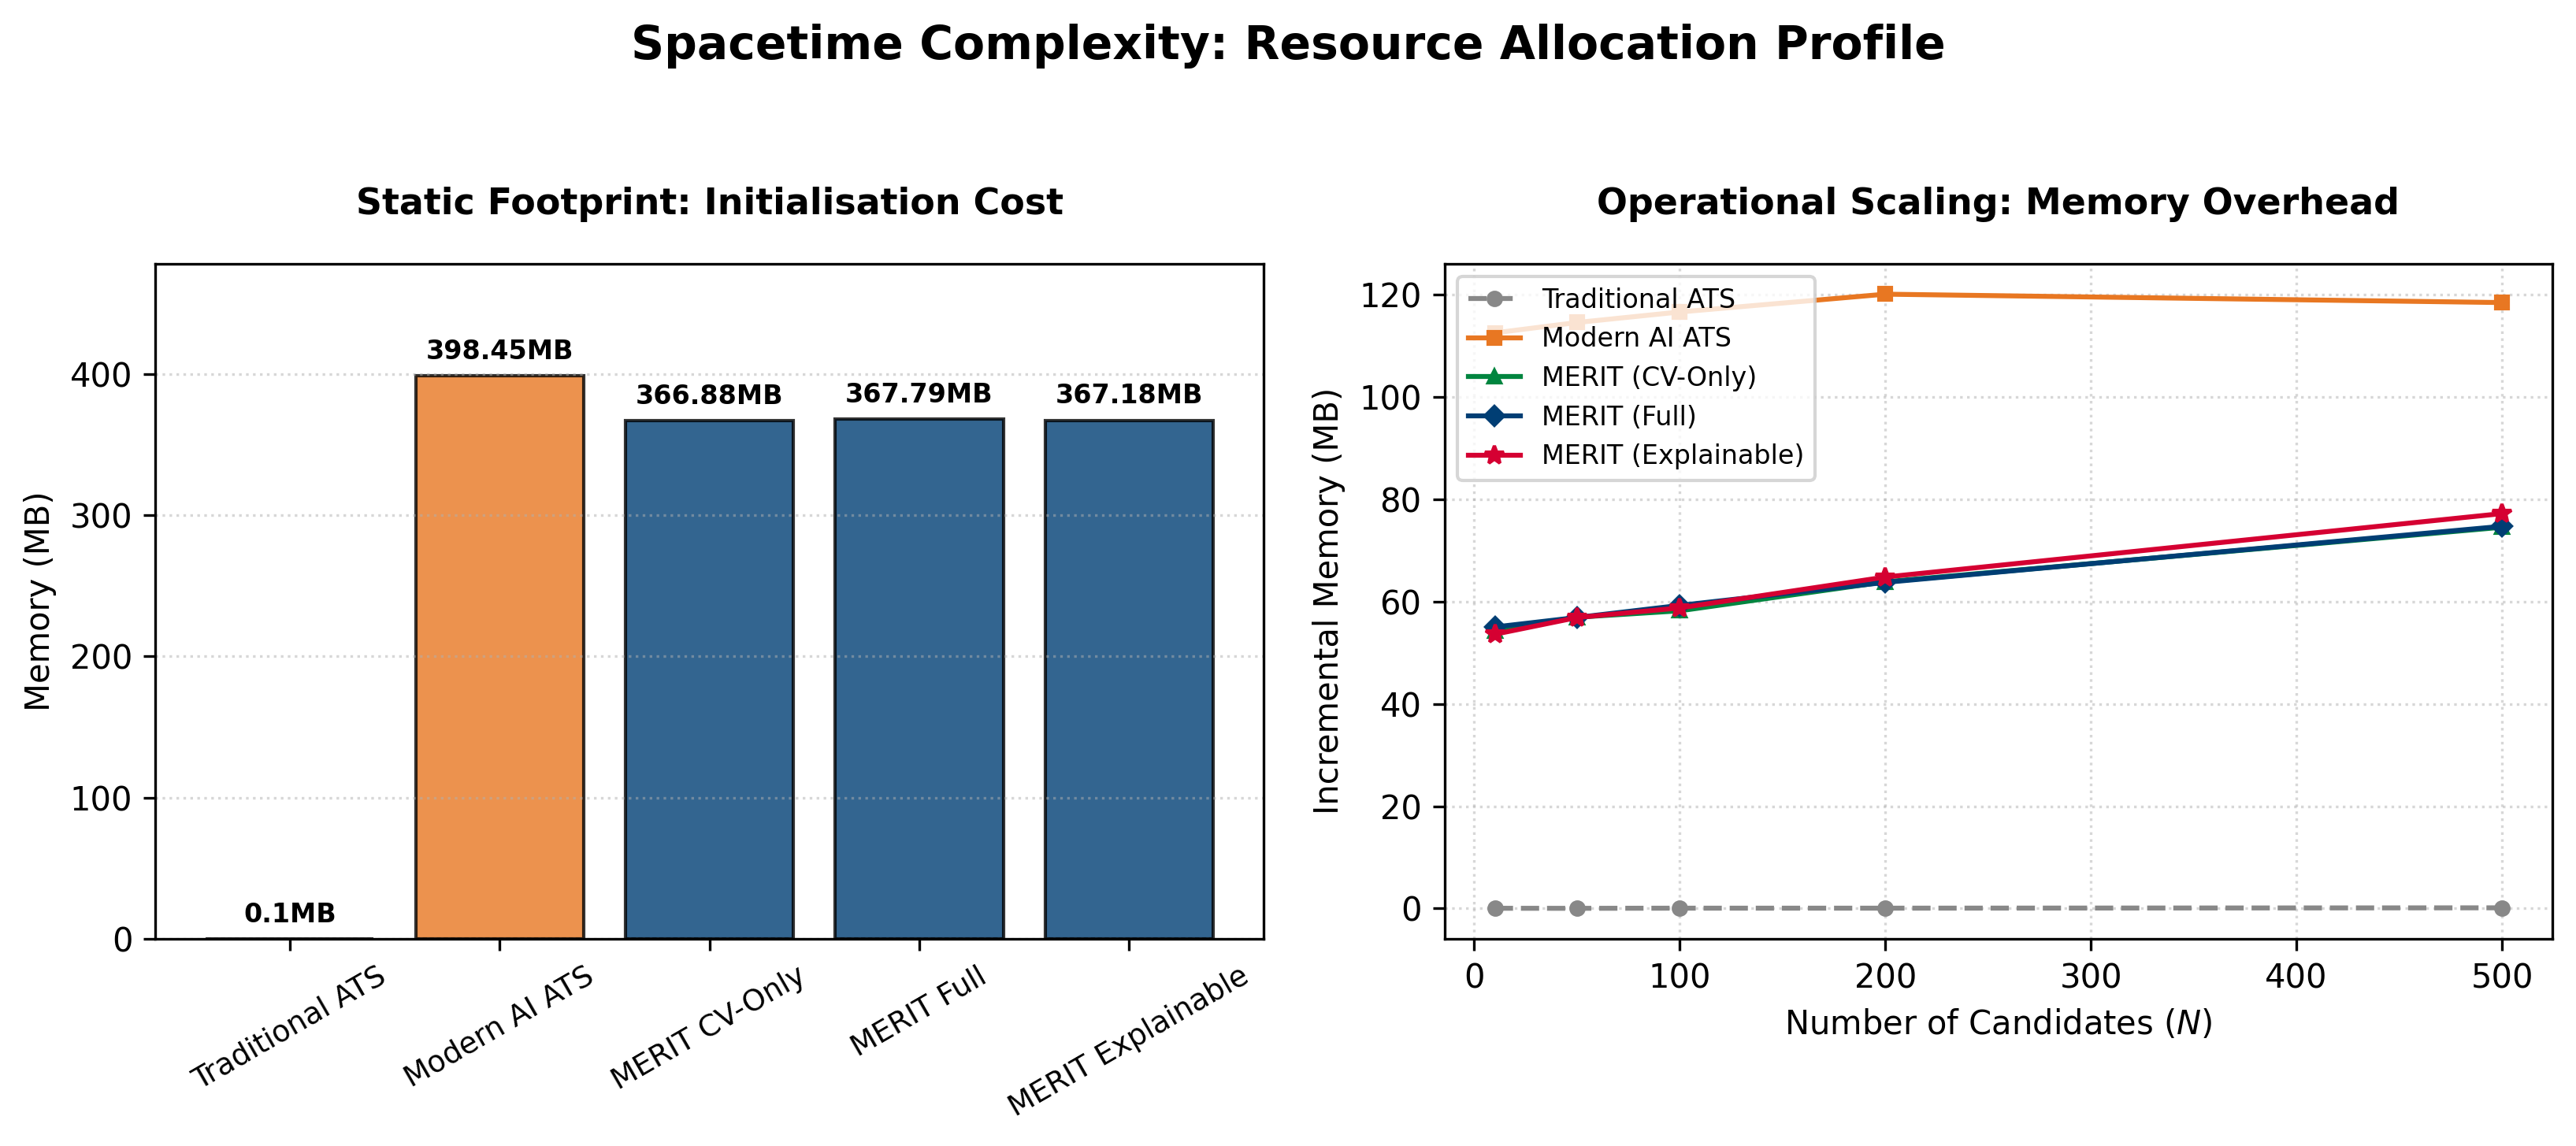
\includegraphics[width=0.98\textwidth]{../evaluation/03-spacetime_study/output/spacetime_complexity_composite.png}
    \caption{Spacetime complexity profile (Study~03). \textbf{Left:} static initialisation footprint. \textbf{Right:} incremental memory overhead vs.\ batch size.}
    \label{fig:spacetime-composite}
\end{figure}
